\chapter{Magnetic Resonance Imaging}
\chaptermark{Magnetic Resonance Imaging} \label{Chp:MRI}

The scope of this chapter includes: 1) physical principles of nulcear magnetic resonance (\acs{NMR}) and magnetic resonance imaging (\acs{MRI}); 2) k-space (spatial-frequency-domain) sampling trajectories and requirements; 3) two important imaging sequences, gradient echo and spin echo; 4) the fundamental image reconstruction algorithm for arbitrary trajectories; and 5) the parallel imaging technique and MRI system. For detailed explanations, please refer to the books by Haacke et al.~\cite{1999_MRI}, Lauterbur et al.~\cite{2000_MRI_Liang}, Bernstein et al.~\cite{2004_MRI_Bernstein}, and Nishimura \cite{2010_principle_mri}.

\section{Nuclear Magnetic Resonance}
Both Felix Bloch and Edward Mills Purcell discovered the phenomenon of NMR in 1946 \cite{1946_NMR_Purcell,1946_NMR_Bloch}, thereby awarded the 1952 Nobel Prize for Physics. The NMR experiment is composed of three fundamental elements: nuclear spin, magnetic field, and resonance.

Firstly, the atomic nucleus, consisting of protons and neutrons, carries an intrinsic angular momentum called \textbf{spin}. Spins of those nuclei with even numbers of protons and neutrons sum up as zero. In contrast, the nuclei, which contain odd numbers of protons and/or neutrons, i.e., $^{1}H$, $^{13}C$, and $^{31}P$, have residual spins. Among these nuclei with spins, hydrogen ($^{1}H$) has been used in MRI most frequently because biological tissues such as water and fat contain many hydrogen atoms. One property of these nuclei is that the spin angular momentum ($\vec{S}$) creates a magnetic moment ($\vec{\mu}$),
\begin{equation}
  \vec{\mu} = \gamma \vec{S} 
\end{equation}
where $\gamma$ is the gyromagnetic ratio. In the absence of any external magnetic field, the nuclear spins act as cylindrical bar magnets with random directions and thus an ensemble (e.g.~one voxel) of spins yields a null net magnetization.

Secondly, in the presence of a static magnetic field $\vec{B}_0$, the $^{1}H$ spins are split into two energy states -- parallel and anti-parallel to $\vec{B}_0$ (corresponding to the lower and higher energy state, respectively), known as Zeeman splitting. According to the Boltzmann relationship, more spins are aligned parallel than those anti-parallel to $\vec{B}_0$ in the thermodynamic equilibrium, resulting in an \textbf{equilibrium net magnetization} ($\vec{M}_0$) 
\begin{equation}
  \vec{M}_0 = \rho \frac{\gamma^{2} \hbar^{2}}{4 k_{b} T} \vec{B}_0
\end{equation}
with $\rho$ the proton density (\acs{PD}) of the spin ensemble, $\hbar$ the Planck constant divided by $2\pi$, $k_B$ the Boltzmann constant, and $T$ the temperature. Here, $\vec{M}_0$ is in the direction parallel to $\vec{B}_0$, defined as the longitudinal ($z$) direction, orthogonal to which is the transversal ($x$-$y$) plane. Moreover, $\vec{M}_0$ precesses about the $z$ axis with a characteristic angular frequency, known as the \textbf{Larmor frequency}
\begin{equation}
  \omega_0 = \gamma \cdot \abs{\vec{B}_0} \quad .
\end{equation}

Thirdly, to generate the NMR phenomenon, a radio-frequency (\acs{RF}) pulse ($\vec{B}_{1}$) with the Larmor frequency is applied in the $x$-$y$ plane to excite the spins, altering the magnetic filed as following 
\begin{equation}
  \vec{B}(t) = \vec{B}_0 + \vec{B}_{1} (t) = 
  \left( \begin{array}{c} 
    0 \\
    0 \\
    \abs{\vec{B}_0}
  \end{array} \right) + 
  \left( \begin{array}{c} 
    \abs{\vec{B}_{1} (t)} \cdot \sin(\omega t) \\
    \abs{\vec{B}_{1} (t)} \cdot \cos(\omega t) \\
    0
  \end{array} \right) \quad .
\end{equation}
The RF excitation flips $\vec{M}_0$ towards the $x$-$y$ plane by a flip angle ($\alpha$),
\begin{equation}
  \alpha = \int_{0}^{t_{\text{RF}}} \gamma \vec{B}_{1} (t) \text{d} t
\end{equation}
with $t_{\text{RF}}$ the RF-pulse duration. For the convenience of illustration, the flip angle used in \cref{Fig:mri-nmr} is \ang{90}. Immediately after the RF excitation, the spin system starts to precess till reaching the equilibrium state again. During this process, antennas (i.e., receiver coils) are used to receive signals from the precessing magnetization in the $x$-$y$ plane. The \textbf{precession} in NMR can be characterized by two intrinsic relaxations, described by the Bloch equation \cite{1946_NMR_Bloch}
\begin{equation} \label{Equ:mri_bloch}
  \frac{\text{d}}{\text{d} t} \vec{M} = \gamma \vec{M} \times \vec{B} + 
  \left( \begin{array}{c} 
    - M_{x} / T_2 \\
    - M_{y} / T_2 \\
    ( M_{0,z} - M_{z} ) / T_1
  \end{array} \right)
\end{equation}
where \acs{T1} is the \textbf{spin-lattice relaxation time} describing the magnetization recovery in the $z$ direction, and \acs{T2} is the \textbf{spin-spin relaxation time} describing the magnetization decay in the $x$-$y$ plane. $T_1$ time constant characterizes the energy exchange between the spin system and the surrounding chemical environment, while both energy exchange with the environment and the dephasing effect of spins are encountered in $T_2$ time constant, which, as a result, is smaller than $T_1$. As spins within the ensemble may exist in different microscopic chemical environments, they precess with different Larmor frequencies, resulting in spin dephasing.

On the other hand, $M_{x}$ and $M_{y}$ in \cref{Equ:mri_bloch} are the magnetization components in the $x$ and $y$ axis, respectively. They are usually written as one single vector, $\vec{M}_{\perp} (t) = M_{x} (t) + i M_{y} (t)$. Moreover, $\vec{B} (t) = \vec{B}_0$ after the RF excitation. Therefore, \cref{Equ:mri_bloch} with regarding to $\vec{M}_{\perp} (t)$ and $\vec{M}_{z} (t)$ can be given as
\begin{align}
  \frac{\text{d} M_{\perp}(t)}{\text{d} t} &= - \frac{M_{\perp}(t)}{T_2} \\
  \Rightarrow M_{\perp}(t) &= M_{\perp}(0) \cdot e^{-t/T_2} \label{Equ:mri_T2} \quad , \\
\intertext{and} 
  \frac{\text{d} M_{z}(t)}{\text{d} t} &= - \frac{M_{z}(t) - M_{0,z}(t)}{T_1} \\
  \Rightarrow M_{z}(t) &= M_{0,z} + [ M_{z}(0) - M_{0,z} ] \cdot e^{-t/T_1} \label{Equ:mri_T1} \quad .
\end{align}
Here, $M_{\perp}(0)$ and $M_{z}(0)$ are the transversal and longitudinal magnetization immediately after the RF excitation, respectively. $M_{0,z}$ is the $z$ component of $\vec{M}_0$. Noteworthy, both time constants vary among biological tissues, rendering different signal intensities in MRI.

\begin{figure}[tb]
  \centering
  \includegraphics[width=1.0\textwidth]{fig/mri-nmr.png}
  \caption{Illustration of a pulsed NMR experiment on a net magnetization $\vec{M}$: equilibrium, excitation, and precession in the presence of a static magnetic field $\vec{B}_0$.} \label{Fig:mri-nmr}
\end{figure}


\section{Spatial Encoding} \label{Sec:mri-signal-detect}
Once the flipped magnetization starts to precess towards its thermodynamic equilibrium, receiver coils detect an electromotive force (EMF) because they are swept by the magnetized nuclear spins and hence create time-varying currents, which eventually become a meaningful image of the sample. As derived in \cite{1999_MRI},
\begin{align} 
  y(t)  &= -\frac{\text{d}}{\text{d}t} \int_{V} \vec{M} (\vec{r},t) \cdot \vec{B}_{\text{coil}} (\vec{r}) \text{d}^{3} r \nonumber \\
  &\propto \omega_0 \int_{V} \vec{M}_{\perp} (\vec{r},t) c(\vec{r}) e^{- i \omega_0 t} \text{d}^{3} r \label{Equ:mri_emf}
\end{align}
where $V$ denotes the excited volume, and the first term ($\omega_0$) reveals that the Larmor oscillations in the $x$-$y$ plane cause the dominant signal in the receiver coil $c(\vec{r})$. Signals from \cref{Equ:mri_emf}, however, cannot distinguish the excited spatially-varying samples. Thus, magnetic-field gradients are used for the purpose of 2D or 3D imaging. 

First of all, the \textbf{slice selection gradient} (e.g.~$G_z$ as shown in \cref{Fig:mri-slice-sel}) is applied during the RF excitation pulse,
\begin{equation} \label{Equ:mri_slice}
  \gamma \vec{B} = \gamma \vec{B}_0 + \gamma \vec{G} \cdot \vec{r} = \left( \begin{array}{c} 
      0 \\
      0 \\
      \omega_0
    \end{array} \right) + \gamma \cdot \left( \begin{array}{c}
      G_x \\
      G_y \\
      G_z
    \end{array} \right) \cdot \left( \begin{array}{c}
     x \\
     y \\
     z
    \end{array} \right)
\end{equation}
where $\vec{r}$ represents the spatial coordinate of $\vec{M}$ and the altered Larmor frequency ($\omega_z = \omega_0 + \gamma G_{z} z$) linearly changes over the longitudinal direction. In principle, an arbitrarily-oriented slice can be selected by appropriately projecting $G_z$ onto $G_x$, $G_y$, and $G_z$ via a \num{3x3} rotation matrix. On the other hand, in order to select a rectangle-shape slice, which corresponds to a rectangular RF pulse in the spatial frequency domain, the applied RF pulse in the time domain must be a sinc function, as the Fourier transform of a rectangle is a sinc, which is ideally infinite but not applicable in practice. A practical solution is to use the truncated-sinc RF pulse.
\begin{figure}[tb]
  \centering
  \includegraphics[width=1.0\textwidth]{fig/mri-slice-sel.png}
  \caption{Slice selection: (Left) The application of a truncated sinc RF pulse and slice selection gradient in time domain. (Right) The relation between the selected slice and Larmor frequency.} \label{Fig:mri-slice-sel}
\end{figure}

Second, two \textbf{frequency encoding gradients} ($G_x$ and $G_y$ here) are used to encode signals from every voxel within the selected slice. Similar to \cref{Equ:mri_slice}, the spatial frequency on the selected slice becomes
\begin{equation} \label{Equ:mri_freq}
  w_{\perp} = \gamma G_x \cdot x + \gamma G_y \cdot y
\end{equation}
which can be inserted into \cref{Equ:mri_emf} and yields
\begin{equation} \label{Equ:emf_grad}
  y(t) \propto \omega_0 \int_{V} M_{\perp} (\vec{r},t_{\text{RF}}) \cdot c(\vec{r}) \cdot e^{- i [\omega_0 + \gamma x \int_{0}^{t} G_x(\tau) \text{d}\tau + \gamma y \int_{0}^{t} G_y(\tau) \text{d}\tau] t } \text{d}^{3} r
\end{equation}
where $M_{\perp}(\vec{r}, t_{\text{RF}})$ denotes the transversal magnetization immediately after the RF excitation, while the first ($\omega_0$) and the RF phase ($e^{-i \omega_0 t}$) term is technically removed by retaining the envelope of the detected signal and using a low-pass filter, respectively. Therefore, the spatial-frequency MR signal encoding, known as the k-space sampling, can be simplified as
\begin{equation} \label{Equ:mri_signal}
  y(t) = \int_{V} M_{\perp}(\vec{r}) \cdot c(\vec{r}) \cdot e^{-i 2\pi \cdot \vec{k} (t) \cdot \vec{r}} \text{d} \vec{r}
\end{equation}
where 
\begin{equation} \label{Equ:mri_ktrj}
  \vec{k} (t) := \frac{\gamma}{2\pi} \int_{0}^{t} \vec{G} (\tau) \text{d} \tau
\end{equation}
denoting the k-space sampling trajectory, and $M_{xy}(\vec{r}, t_{\text{RF}})$ is equivalent to \acs{PD}. It can be seen that the received signal in k-space is the Fourier transform of the dot product between PD and the coil sensitivity map.



\section{Imaging Sequences} \label{Sec:mri-seq}
To begin with, it is important to introduce the free induction decay (\acs{FID}), the received NMR signal immediately after the RF excitation, as shown in \cref{Fig:mri-fid}. The envelope of the FID can be approximated by an exponential function with an effective spin-spin relaxation time (\acs{T2s}), 
\begin{equation} \label{Equ:mri_t2s}
  \frac{1}{T_{2}^{*}} = \frac{1}{T_2} + \gamma \cdot \Delta B_0
\end{equation}
where $\Delta B_0$ is the local magnetic field inhomogeneity. Thereby, $T_{2}^{*}$ is even shorter than $T_2$.
\begin{figure}[tb]
  \centering
  \includegraphics[width=0.6\textwidth]{fig/mri-fid.png}
  \caption{Free induction decay. The oscillating solid line represents the received signal, whose envelop (gray) is the $T_{2}^{*}$ exponential decay curve.} \label{Fig:mri-fid}
\end{figure}

\subsection{Gradient Echo}
A typical spoiled gradient echo sequence for 2D imaging is shown in \cref{Fig:mri-seq-ge-cart}, where one repetition block encodes one echo in k-space. Here, the application of the prephasing gradient adds a spatially-dependent phase term to nuclear spins, which accelerates the FID signal decay because this gradient perturbs the static magnetic field $\vec{B}_0$, produces spatially-varying field inhomogeneities, and leads to faster spin dephasing. The dephased spins, however, can be rephased by a gradient with reversed polarity, namely the readout gradient, during which the analog-to-digital converter (ADC) is switched on to readout signals. When the area of the readout gradient is equal to that of the prephasing gradient, the signal of the central k-space point ($k_x = 0$) is reached. This time point is named as the echo time (\acs{TE}). The sequence block represents one repetition, whose duration is defined as the repetition time (\acs{TR}).
\begin{figure}[tb]
  \centering
  \includegraphics[scale=1]{fig/mri-seq-ge-cart.png}
  \caption{Spoiled gradient echo sequence diagram. For the simplicity of explanation, the imaging slice is the transversal plane. Thus, the $z$ gradient is used for slice selection, while the $x$ and $y$ gradients are used for readout and phase-encoding gradient, respectively. Phase-encoding gradients effectively separate every readout line along the $k_y$ direction.} \label{Fig:mri-seq-ge-cart}
\end{figure}

A specific example of gradient echo sequences is \acs{FLASH}, invented by Frahm et al.~in 1985 \cite{1986_FLASH}. FLASH is a fast imaging technique that reduces MRI measuring times to about hundreds of milliseconds per image due to its extremely short TE and TR. Moreover, the equilibrium magnetization is only slightly flipped towards the transversal plane by a low flip angle (e.g.~\ang{15}).

\subsection{Spin Echo}
Spin echo was discovered by Hahn in 1950 \cite{1950_spin-echo}. A well-known variant of spin echo sequences that has been widely used in clinics is the rapid acquisition with relaxation enhancement (\acs{RARE}) sequence, invented by Hennig et al.~in 1986 \cite{1986_RARE}. As depicted in \cref{Fig:mri-seq-se-cart}, a \ang{90} RF excitation pulse is applied to flip the equilibrium magnetization to the $x$ axis, then a \ang{180} RF pulse is applied at time $\text{TE}/2$ to flip the dephased spins along the $y$ axis, and after the same time period $\text{TE}/2$ spins will be completely rephased again. In this process, the dephasing effect caused by local magnetic field inhomogeneities is compensated by the \ang{180} pulse. Thus, the signals of spin echoes are weighted by $T_2$, instead of $T_2^*$ in gradient echoes. In general, spin echo sequences produce $T_2$-weighted images, in contrast to $T_1$-weighted images from FLASH with relatively shorter TE and TR.
\begin{figure}[tb]
  \centering
  \includegraphics[scale=1]{fig/mri-seq-se-cart.png}
  \caption{Spin echo sequence diagram. Spin dephasing is compensated by a \ang{180} RF pulse that flips all spins along the $y$ axis (assuming that spins are flipped to the $x$ axis by a \ang{90} RF excitation pulse), and thus all spins refocus again on the $x$ axis at the echo time.} \label{Fig:mri-seq-se-cart}
\end{figure}



\section{k-Space Sampling Trajectories} \label{Sec:mri-ktrj}
\begin{figure}[tb]
  \centering
  \subfloat[][Cartesian]{ %
    \label{Fig:mri-trj-cartes} %
    \includegraphics[width=0.3\textwidth]{fig/mri-trj-cartes.png}} \quad
  \subfloat[][Radial]{ %
    \label{Fig:mri-trj-radial} %
    \includegraphics[width=0.3\textwidth]{fig/mri-trj-radial.png}} \\
  \subfloat[][Spiral]{ %
    \label{Fig:mri-trj-spiral} %
    \includegraphics[width=0.3\textwidth]{fig/mri-trj-spiral.png}} \quad
  \subfloat[][Random]{ %
    \label{Fig:mri-trj-random} %
    \includegraphics[width=0.3\textwidth]{fig/mri-trj-random.png}} %
  \caption{Schematic illustration of four most popular k-space sampling trajectories. The dashed lines in \protect\subref{Fig:mri-trj-cartes} represent the the trajectories generated by the predephasing and the phase-encoding gradients. The solid lines represent the readout echoes. The intersections of blue lines represent the 2D Cartesian grid.}
  \label{Fig:mri-trj}
\end{figure}
\cref{Fig:mri-trj} depicts four most popular k-space sampling trajectories. According to \cref{Equ:mri_ktrj}, the spoiled gradient echo sequence in \cref{Fig:mri-seq-ge-cart} results in the \textbf{Cartesian} sampling trajectory as shown in \cref{Fig:mri-trj-cartes}, where every sample is located on the Cartesian grid. Thus, a fully-sampled Cartesian dataset mainly requires the fast Fourier transform (\acs{FFT}). Moreover, it is insensitive to gradient delay errors, in which case all echoes in Cartesian sampling have identical phase shifts because the same readout gradient is used for every echo.

The \textbf{radial} sampling trajectory, as shown in \cref{Fig:mri-trj-radial}, has been the very first trajectory proposed for MRI by Lauterbur in 1973 \cite{1973_Nature}, but requires more precise gradient switching because gradient delay errors induce inconsistent phase shifts among echoes. According to \cref{Equ:mri_ktrj}, radial sampling can be accomplished with the following readout gradients,
\begin{equation} \label{Equ:mri_grad_rad}
  \begin{aligned}
    G_x &= G_{\text{max}} \cdot \cos(\theta) \\
    G_y &= G_{\text{max}} \cdot \sin(\theta)
  \end{aligned}
\end{equation}
where $G_{\text{max}}$ is the maximal gradient amplitude, and $\theta$ is the angle of one radial echo (\textit{spoke}). 

As shown in \cref{Fig:mri-trj-spiral}, the \textbf{spiral} sampling trajectory \cite{1999_spiral} can be implemented via
\begin{align}
  \vec{k}(t) &= a \cdot \theta (t) \cdot e^{i \theta (t)} \quad \text{with} \; \theta (t) = \frac{t}{\sqrt{\alpha + (1 - \alpha) \cdot t}} \quad ,  \label{Equ:mri_grad_spi} \\
\intertext{and}
  \vec{G}(t) &= \frac{2\pi}{\gamma} \frac{\text{d}}{\text{d}t} \vec{k}(t) \quad .
\end{align}
Its characteristics were reviewed by Block et al.~in 2005 \cite{2005_spiral_JMRI}. When compared to other k-space sampling trajectories, spiral sampling has longer readouts, which are prone to field-inhomogeneity-induced phase errors. 

The last one is the \textbf{random} sampling trajectory, as shown in \cref{Fig:mri-trj-random}. It receives recent interest because it meets the prerequisite of applying compressed sensing \cite{2006_CS} to MRI image reconstruction -- \textit{incoherent} sampling \cite{2007_Sparse_MRI}. Whereas this scheme is inefficient in 2D trajectories, it can be successfully implemented in combination with 3D sampling schemes, where $G_z$ is also used as a readout gradient and sampled by random ($k_x$, $k_y$) tuples.







\begin{figure}[tb]
  \centering
  \includegraphics[width=0.8\textwidth]{fig/mri-smp-req.png}
  \caption{Discretization of an image and k-space signal. The image is related to its k-space signal by a Fourier transform.} \label{Fig:mri-smp-req}
\end{figure}
\section{Sampling Requirements}
As shown in \cref{Fig:mri-smp-req}, the continuous k-space signal can be discretized via a Dirac comb function $u(k)$ with the sampling distance ($\Delta k$) 
\begin{align}
  \tilde{y}(k) 
  &= y(k) \cdot u(k) \label{Equ:mri_discrete_y}\\
  &= \Delta k \sum_{p=-\infty}^{\infty} y(p \Delta k) \cdot \delta(k - p \Delta k)
\end{align}
where the inverse Fourier transform of $u(k)$ is
\begin{align}
  U(r) 
  &= \int \Delta k \cdot \delta(k - p \Delta k) \cdot e^{i 2\pi \cdot k \cdot r} \text{d} k \\
  &= \sum_{p=-\infty}^{\infty} \Delta k \cdot e^{i 2\pi \cdot p \Delta k \cdot r}
\end{align}
which only has non-zero values when $r = q / \Delta k$, with $q \in [-\infty,\infty]$, and hence is again a Dirac comb function
\begin{equation}
  U(r) = \delta (r - \frac{q}{\Delta k}) \quad .
\end{equation}
Following \cref{Equ:mri_discrete_y}, the corresponding discrete image is
\begin{align}
  \tilde{\rho}(r) 
  &= \mathcal{F}^{-1} \{ y(k) \cdot u(k) \} \\
  &= \rho(r) \ast U(r) \\
  &= \rho(r) \ast \delta (r - \frac{q}{\Delta k})
\end{align}
with $\ast$ the convolution. It can be seen that $\tilde{\rho}(r)$ is an infinite and periodic function with the period
\begin{equation} \label{Equ:mri_fov}
  r_T = 1 / \Delta k := \text{FOV}
\end{equation} 
where the field-of-view (\acs{FOV}), i.e., the selected image plane (e.g.~in \si{\square\mm}), consists of only one period of $\tilde{\rho}(r)$. Moreover, the discrete $\rho(r)$ is composed of thousands of image elements (pixels), whose size ($\Delta r$), typically defined as the spatial resolution, is given as
\begin{equation} \label{Equ:mri_pixel}
  \Delta r = \frac{\text{FOV}}{N} = \frac{1}{\Delta k \cdot N} = \frac{1}{2k_{\text{max}}}
\end{equation}
with $N$ the number of samples per echo and $k_{\text{max}}$ the maximal k-space sampling position. 

Alternatively, according to \cref{Equ:mri_ktrj}, $\Delta k$ can also be written as
\begin{equation} \label{Equ:mri_smp_int}
  \Delta k_x = \frac{\gamma}{2\pi} G_x \Delta t_x \quad \text{and} \quad \Delta k_y = \frac{\gamma}{2\pi} G_y \Delta t_y
\end{equation}
where $\Delta t_x$ and $\Delta t_y$ is the sampling interval (dwell time) along the $G_x$ and $G_y$ direction, respectively. \cref{Equ:mri_smp_int} indicates how much time is required to encode one k-space sample, so the sampling rate is $1 / \Delta k$, which, according to the Nyquist-Shannon sampling theorem, has to satisfy the following condition in order to avoid the image aliasing artifact,
\begin{equation}
  \Delta k = \frac{2 k_{\text{max}}}{N} \leq \frac{1}{\text{FOV}} \quad . 
\end{equation}
Here, the reduction of $\Delta k_x$ along the readout direction does not increase the measuring time but enlarges the aliasing-free area. 

Further, $\Delta k$ in \cref{Equ:mri_smp_int} is determined by two factors: the gradient strength and the dwell time. For fixed $\Delta k$ and $k_{\text{max}}$, a reduced gradient strength prolongs the dwell time and also the total readout duration, yielding a higher signal-to-noise ratio (SNR). The reciprocal of $\Delta t$ is represented by the receiver bandwidth (\acs{BW}). Therefore, the higher the bandwidth, the faster the sampling rate, and the lower the \acs{SNR} \cite{2009_Zhang_Thesis}. 


\section{Gridding \& FFT Image Reconstruction} \label{Sec:mri_grid}
In the case of Cartesian sampling, an inverse \acs{FFT} can be directly applied to the sampled k-space data to obtain an image. For non-Cartesian sampling trajectories (e.g.~radial and spiral), however, the sampled k-space data are not necessarily located on the Cartesian grid. As a result, the image reconstruction of k-space data from non-Cartesian sampling requires the non-uniform FFT (\acs{NUFFT}) \cite{2003_NUFFT}, known as the \textbf{gridding} algorithm in MRI \cite{1991_conv_gridding,1999_gridding_TMI,2005_gridding,2008_Block_Thesis}, to interpolate the data onto the Cartesian grid prior to the uniform inverse FFT. In principle, the gridding algorithm includes the following steps
\begin{enumerate}
\item Density compensation. As the sampling density in non-Cartesian trajectories may not be equally distributed in k-space, so a density compensation function (DCF) is required to properly weight every k-space data;
\item Convolution. The density-compensated data is convolved with a window function (e.g.~the Kaiser-Bessel function) with a finite width to interpolate every sample onto its neighboring Cartesian grid, whose minimal sampling distance ($\Delta k_{\text{min}}$) of the Cartesian grid can be smaller than that ($\Delta k$) of the non-Cartesian sampling trajectory. The ratio between them is denoted as the over-gridding ratio $o = \Delta k / \Delta k_{\text{min}}$, which is helpful in reducing image aliasing artifacts;
\item Roll-off correction. Note that the convolution in k-space in the previous step is equivalent to a dot product between the object and the inverse FFT of the window in image domain. Thus, a reconstructed image is obtained by a 2D inverse FFT of the gridded data and then divided by the inverse Fourier transform of the window function. Finally, the image is cropped according to the over-gridding ratio.
\end{enumerate}



\section{Parallel Imaging} \label{Sec:mri_pi}
One main problem in MRI is the imaging speed. Even with the Cartesian FLASH sequence, about one second is required to obtain one image. This temporal resolution is not fast enough for the study of fast physiological motions, e.g.~beating heart. To speed up MRI, data undersampling is a feasible approach, but undersampled k-space results in aliased images. To overcome this problem, parallel imaging has been of great interest ever since the development of phased-array coils \cite{1990_phased_array}, which are usually placed around the subject in order to simultaneously receive k-space data. 

As shown in \cref{Fig:mri-pi}, the coils are more sensitive to signals near to their locations. The spatially-varying sensitivities of the coils are named the \textbf{coil sensitivity map}, in correspondence to which even the aliased coil images due to the two-fold undersampling exhibit brighter intensities in respective regions. This is a direct indication that parallel imaging with multiple receiver coils creates redundant information which can be used to estimate an un-aliased image and hence eventually accelerates data acquisition. The forward operation in parallel imaging can be mathematically denoted as
\begin{equation} \label{Equ:mri-pi-forward}
  F: x \mapsto \left( \begin{array}{c}
    P \mathcal{F} \{ \rho \cdot c_1 \} \\
    \vdots \\
    P \mathcal{F} \{ \rho \cdot c_N \} \\
  \end{array} \right)
\end{equation}
where $\rho$ is the image, $c_n$ is the $n^{\text{th}}$ coil sensitivity map, $\mathcal{F}$ is the 2D FFT, and $P$ is the sampling pattern. On the contrary, the task of the inverse problem posed by parallel imaging is to estimate an un-aliased image and/or a set of coil sensitivity maps via the undersampled multi-coil data and the sampling pattern.
\begin{figure}[tb]
  \centering
  \includegraphics[width = 1.0\textwidth]{fig/mri-pi.png}
  \caption{Schematic illustration of parallel imaging. The forward model can be understood as the 2D FFT ($\mathcal{F}$) of the dot product between the image $\rho$ and every coil sensitivity map evaluated on the sampling pattern. In case of undersampling (as depicted in the sampling pattern, two-fold undersampling is used here), the direct FFT gives aliased coil images. Inverse problem is to estimate an un-aliased image and/or coil sensitivity maps given the undersampled multi-coil data and the sampling pattern.} \label{Fig:mri-pi}
\end{figure}

There exists three generic reconstruction techniques for parallel imaging, sensitivity encoding (\acs{SENSE}) \cite{1999_SENSE,2001_gSENSE}, simultaneously acquisition of spatial harmonics (\acs{SMASH}) \cite{1997_SMASH}, and generalized autocalibrating partially parallel acquisitions (\acs{GRAPPA}) \cite{2002_GRAPPA}, all of which have been commercialized and used in routine clinic. 

The generalized SENSE treats parallel imaging as a linear inverse problem which intends to optimize the following cost function
\begin{equation} \label{Equ:mri_inv_cost}
  \Phi(x) = \argmin\limits_x \sum_{n=1}^{N} \norm{y_n - F(\rho \cdot c_n)}_2^2 + \alpha \norm{\rho}_2^2 \quad \text{with} \; x = \rho \quad .
\end{equation}
Prior to solving this function, the coil sensitivity maps need to be calculated via either a calibration scan or the auto-calibration signal (\acs{ACS}). ACS is usually accomplished by fully sampling the low-spatial-frequency region while the rest of k-space remains undersampled according to the user-defined reduction factor $R$. Non-Cartesian trajectories such as spiral and radial, however, offer inherent self-calibrating signals due to their densely sampled center \cite{2005_self_cal_pi}. With coil sensitivity maps, the above function can be solved by conjugate gradient (\acs{CG}) method and thus this method is dubbed as CG-SENSE. Moreover, due to the ill-condition of the inverse problem, Tikhonov regularization that penalizes the $L^2$ norm of the estimate image is used. 

Recent progress in compressed sensing \cite{2006_CS} has enabled the application of $L^1$-norm regularizations into SENSE-type iterative image reconstructions. $L^1$-norm regularizations are preferable for estimating sparse images, which are achievable via incoherent sampling and sparsifying transforms (e.g.~wavelet). As a result, $L^1$-norm regularizations produce fewer coefficients with non-zero values due to the stronger penalties on small-value coefficients compared to $L^2$-norm regularizations. 

One important variant of SENSE is $k$-$t$ SENSE \cite{2003_k-t_SENSE}, proposed by Tsao et al.~in 2003 for dynamic imaging with high frame rates. Here, $k$ and $t$ refer to the phase-encoding index and acquisition time, respectively. With 1D FFT on $k$ and $t$ respectively, the data in $x$-$f$ space can be obtained. $k$-$t$ SENSE consists of two reconstruction steps. The first step is named the training stage, where a dataset in the low spatial frequency region is acquired and then a signal covariance matrix in $x$-$f$ space is determined. This matrix is considered to be consistent and is thereby used in the second step (acquisition stage) to reconstruct undersampled data.

In contrast, both SMASH and GRAPPA are based on the assumption that a k-space data point is highly correlated with its neighbors, so the missing data can be a linear combination of neighboring signals with appropriate weights. The weights are determined by fitting undersampled k-space data to the ACS. Afterwards, both the undersampled data used in the fitting and the weights are utilized to composite the missing data. GRAPPA-type image reconstructions result in uncombined coil images, which can be combined via either sum of squares \cite{1990_phased_array} or phase-preserving coil combination algorithms \cite{2000_coil_comb}.


\section{MRI System}
As shown in \cref{Fig:mri-sys}, the studies presented in this thesis were conducted at a commercial scanner (MAGNETOM Prisma, Siemens Healthcare\footnote{\url{www.healthcare.siemens.com}}, Erlangen, Germany) with a superconducting magnet of field strength $\abs{\vec{B}_0} = \num{3}$~Tesla (\si{\tesla}) and two built-in body coils for RF excitation and signal receiving. Moreover, the gradient system has a maximal gradient strength of \SI{80}{\milli\tesla\per\meter}. For the gradient switching, the raster time can be as fast as \SI{10}{\micro\second}, and the maximal slew rate is \SI{200}{\tesla\per\meter\per\second}. In addition, the receiver coils used are the \num{64}-channel head coil, the \num{18}-element thorax coil, and the \num{32}-channel spine coil.
\begin{figure}[tb]
  \centering
  \includegraphics[width = 1.0\textwidth]{fig/mri-sys.png}
  \caption{(Left) MRI system and (right) receiver coils. (Top right) 64-channel head coil and (bottom right) 18-element thorax coil.} \label{Fig:mri-sys}
\end{figure}


